\section{ANALISIS E INTERPRETACION DE RESULTADOS} 
En el presente laboratorio se ha desarrollado un proyecto llamado "AlumnosWebApp" de tipo Web Application, usando la Web API para realizar con ello el servicio de REST.
Este proyecto trata acerca de calificar las tareas de los alumnos, haciendo primero el resgistro de los alumnos y sus tareas para luego relacionar las tareas con los alumnos correspondiente y de modo el cual se podrá poner una calificación.
Se utilizaron tres clases, una para la crecion del "Alumno" , otra para la creacion de la "Tarea" con sus respectivos atributos y otra clase de "TareaAlumno", que esta útima se llama al atributo de IdTarea y IdAlumno, aparte de sus atributos respectivos, para que se relacionen y se califique la tarea del alumno.
\\
Por medio de los controladores se usará la Web API por el cual podremos acceder a la web mediante el protocolo HTTP.
Una ves que tenemos el codigo listo, se para a verificar que el proyecto funcione con el servicio de Rest, que nos permiten listar, crear, leer, actualizar y borrar información.
Cuando solicitamos una pagina web, podemos hacer por diferentes métodos, el mas común es el GET, es el que usamos cuando digitamos una dirección en nuestro navegador, en ocasiones utilizamos POST, cuando enviamos un formulario con datos, pero las aplicaciones pueden usar otros métodos como PATCH, PUT, etc.
\begin{itemize}
\item Listar y leer: Usan el método GET
\item Crear: Usan el método POST
\end{itemize}
Para validar el funcionamiento, primero se ejecuta el proyecto y vemos observamos que formato de la cadena hay que seguir para probar en Postman, que es una herramienta que permiten realizar tareas diferentes dentro del mundo API REST. 
\begin{center}
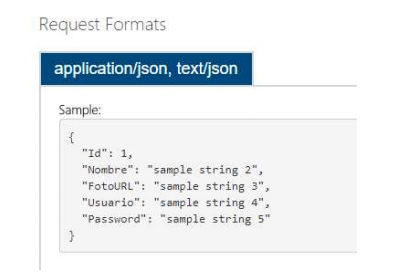
\includegraphics[width=5cm]{./Imagenes/analisis1}
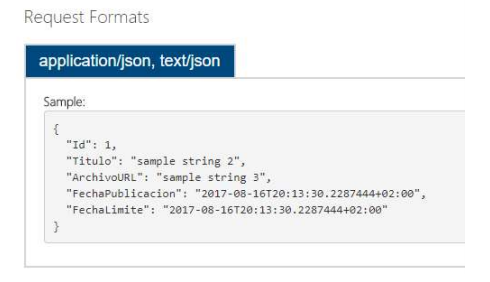
\includegraphics[width=5cm]{./Imagenes/analisis2}
\end{center}
Realizamos primero la creacion de un alumno, siguiendo el formato de la caden. Para crear un alumno usamos la operación de POST y para verifiCar si se ha creado el alumno, realizamos la operacion de GET; y lo mismo para el caso de la tarea.
Aqui se puede notar como se ha realizado correctamente el registro de ambos casos a través del servicio de REST y ahora lo que falta es vincular el alumno con su tarea y calificarla.
\\ Para realizar la calificación de la tarea del alumno se sigue la primera parte del formato de cadena y ahi se coloca tanto el indice del alumno como de la tarea y los datos correspondientes a la calificación, usando la operación de POST.
\begin{center}
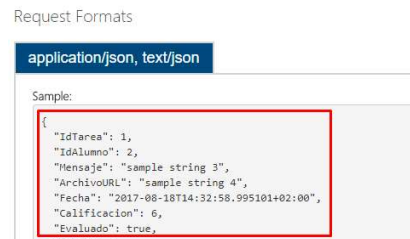
\includegraphics[width=5cm]{./Imagenes/analisis3}
\end{center}
Una vez realizada el registro de la calificación de la tarea del alumno con la operación GET podemos revisar si ha sido verdaderamente registrada. Gracias a estas operaciones de GET POST utilizadas la transferencia de datos en un sistema REST facilita la existencia de una interfaz uniforme que sistematiza el proceso con la información.